\documentclass{article}

% ICBINB 2026 style (workshop template, double-blind track).
\usepackage[dblblindworkshop]{neurips_2026}
\workshoptitle{I Can't Believe It's Not Better (ICBINB): Failure Modes of AI in Biology}
\raggedbottom
\setlength{\textfloatsep}{3pt plus 2pt minus 2pt}
\setlength{\floatsep}{2pt plus 1pt minus 1pt}
\setlength{\intextsep}{1pt plus 1pt minus 1pt}

\usepackage[utf8]{inputenc}
\usepackage[T1]{fontenc}
\usepackage{hyperref}
\usepackage{url}
\usepackage{booktabs}
\usepackage{amsfonts}
\usepackage{nicefrac}
\usepackage{microtype}
\usepackage{xcolor}
\usepackage{graphicx}
\usepackage{subcaption}
\usepackage{amsmath}
\usepackage{amssymb}
\usepackage{mathtools}

\title{TopK Sparsity Costs Predictive Power and Overfits Its Own Selection Procedure at Low K}

\author{%
  Anonymous Author(s) \\
  Affiliation \\
  Address \\
  \texttt{email} \\
}

\begin{document}

\maketitle

\begin{abstract}
Sparse autoencoders (SAEs) are increasingly used to decompose biological foundation models into interpretable features. This carries an implicit assumption: since reconstruction fidelity can be pushed arbitrarily high, a sparse representation should be a safe stand-in for the dense representation it was trained on. We test this assumption in a concrete, practically motivated drug-discovery setting---filtering poor docking poses from a physics-informed protein-ligand docking pipeline's variational autoencoder latent space, across a sweep of sparsity levels---and find that it does not hold. Dense latents consistently match or outperform sparse autoencoder representations on pose-quality classification, even at sparsity levels where reconstruction is nearly perfect. Separately, pose filters built from the sparsest, and by the usual argument most interpretable, representations pass their own selection procedure but systematically fail to generalize to held-out data, while less aggressively sparse representations hold up reliably. Both point to a shared explanation: TopK's magnitude-based feature selection discards classifier-relevant information and leaves individual features with too few examples for reliable selection-set statistics. The practical caution for anyone deploying SAE-based filters in biological pipelines is direct: reconstruction fidelity and feature-level interpretability are not proxies for downstream predictive power or selection reliability, and both must be checked directly, on the actual probe and selection procedure in use, at every sparsity level under consideration, before deployment.
\end{abstract}

\section{Introduction}

Predicting how a ligand binds a flexible protein target, the induced fit docking (IFD) problem \citep{sherman2006}, is one of computational biochemistry's hardest problems: a ligand and a flexible receptor must be co-optimized against each other, and induced-fit effects that rigid-receptor docking ignores routinely make or break a pose's accuracy \citep{miller2021}. Interpretability is not a purely academic concern here: understanding \emph{why} a model scores a pose highly is treated as being as important as the score itself for trustworthy deployment in drug discovery \citep{dhakal2022,sim2025,qadri2025}. Structure-informed, physics-grounded pipelines are an active area partly for this reason---they promise more interpretable, more generalizable predictions than end-to-end sequence-to-structure models \citep{wu2025,lam2025,jiang2026}.

Sparse autoencoders (SAEs) decompose opaque neural representations into interpretable, monosemantic features \citep{templeton2024,gao2024,bricken2023}. Applied to protein language models, they have already recovered biologically meaningful structure---secondary structure, binding sites, evolutionary conservation \citep{adams2025,simon2025}---and the same approach has since been extended to structure-generation and protein-folding representations \citep{zarzecki2025,parsan2025,yu2026}. This growing body of positive results shares an implicit assumption: decomposition comes cheaply. An SAE with enough hidden units and a small enough sparsity constraint can, in principle, reconstruct the dense representation almost perfectly. Scaling studies back this up directly, reporting clean, predictable reconstruction-vs-sparsity tradeoff curves as autoencoder width and $K$ grow \citep{gao2024}. Under this assumption, any information present in the dense representation should still be recoverable from the sparse one, and performance on a downstream task built from the sparse representation should be no worse than performance built directly from the dense latent, at least once reconstruction fidelity is reasonably high. That expectation is borne out in at least one recent case, where downstream linear probes fit in an SAE's sparse latent space matched or exceeded probes fit directly on the dense representation \citep{yu2026}.

We tested this expectation in the Friesner Group's IFD-ML, a physics-informed protein-ligand docking pipeline that combines induced-fit docking \citep{sherman2006,miller2021,li2011} with a VAE and diffusion-based conformational sampling, achieving strong performance in cross-docking benchmarks similar to \citet{mansoor2024}. It generates thousands of candidate poses per complex, each represented by a 30-dimensional continuous VAE latent vector, and each requiring expensive downstream energy minimization regardless of quality \citep{li2011}.

A natural, practically valuable use of an SAE trained on this latent space is a pre-refinement filter: use SAE-derived features, rather than the raw latent, to flag likely-poor poses before they consume refinement compute. This requires two things to hold: the SAE representation should support pose-quality classification at least as well as the raw latent, and a filter selected on held-out data should generalize reliably to a separate test set. We test both across a realistic sweep of sparsity levels and find that neither holds: (1) raw latents match or beat every trained SAE on classification, even at sparsity levels with near-perfect reconstruction; and (2) filters built from the sparsest, and by the field's standard most interpretable, representations pass their own selection procedure but fail to generalize to held-out data, while less aggressively sparse representations hold up reliably.

\section{Methodology}

We trained TopK SAEs \citep{adams2025} on 435{,}069 docking poses across 36 protein-ligand systems, split by case (not pose) into $\sim$70/15/15 train/validation/test to prevent leakage. Each SAE uses a $4\times$ expansion (30D input $\to$ 120D hidden $\to$ 30D reconstruction); the TopK operation keeps only the $K$ largest hidden activations per example and zeros the rest, with reconstruction loss as the sole training objective. The pre-encoder bias is initialized to the training-set mean of normalized activations and subtracted before encoding, following \citet{simon2026}'s dead-feature mitigation. We swept $K\in\{1,3,6,8,15,20,30\}$, 5 seeds per $K$, selecting the best run per $K$ by validation loss.

We evaluated two downstream tasks on the resulting representations, both on a held-out test set never touched during training or selection:

\textbf{Classification.} Logistic regression classifiers (class-balanced) were fit to predict bad-pose vs.\ good-pose (RMSD $\le$ 4\r{A} native-like, following \citet{shim2022}) from (a) the 30D normalized raw VAE latent (L2 penalty) and (b) the 120D SAE activations for each trained $K$ (L1 penalty). We report test-set auPR, our primary metric given the 63.4\% bad-pose base rate.

\textbf{Filtering.} For each $K$, we built a pre-refinement filter using a three-way train/select/test discipline: per-feature F1-maximizing activation thresholds and precision-based candidate ranking (requiring recall $>$0.02 to exclude degenerate picks) were fit on a pooled train+validation selection set; the top 16 candidates were then searched over all subset unions, on that same selection set, for the union maximizing recall subject to retaining $\ge$80\% of native-like (good) poses. The winning union was applied exactly once to test. Here we report what happens when this procedure is applied uniformly across the full $K$ sweep, rather than restricting to the small number of $K$ values a practitioner would ultimately consider deploying.

\section{Results and Discussion}

\subsection{Sparsity provides no consistent classification lift}

Table~\ref{tab:aupr} reports auPR and FVE across the full $K$ sweep. Raw dense latents (auPR 0.770 at the 4\r{A} threshold) beat every trained SAE $K$ at this threshold, including $K$=30, whose FVE reaches 100\%---near-perfect reconstruction does not translate into matching, let alone exceeding, the raw latent's classification performance. FVE grows essentially monotonically with $K$; auPR does not track it at all: $K$=6 (FVE 49.5\%) modestly \emph{outperforms} $K$=15 (FVE 90.0\%) on 2\r{A} auPR, and no $K$ tested closes the gap to the raw latent at either threshold.

\begin{table}[!ht]
\caption{auPR and FVE, raw latents vs.\ SAE $K$ (test set, full sweep).}
\label{tab:aupr}
\centering
\begin{small}
\begin{tabular}{lcccc}
\toprule
Rep. & auPR (4\r{A}) & auPR (2\r{A}) & FVE & Dead \% \\
\midrule
Raw latents & 0.770 & 0.855 & --- & --- \\
SAE $K$=1  & 0.660 & 0.838 & $-$0.2\% & 80.8\% \\
SAE $K$=3  & 0.709 & 0.858 & 33.7\% & 2.5\% \\
SAE $K$=6  & 0.737 & 0.867 & 49.5\% & 0.8\% \\
SAE $K$=8  & 0.719 & 0.821 & 62.0\% & 1.7\% \\
SAE $K$=15 & 0.750 & 0.846 & 90.0\% & 25.8\% \\
SAE $K$=20 & 0.749 & 0.846 & 98.0\% & 30.8\% \\
SAE $K$=30 & 0.742 & 0.810 & 100.0\% & 16.7\% \\
\bottomrule
\end{tabular}
\end{small}
\end{table}

At the 2\r{A} threshold two SAE $K$'s (3 and 6) edge past the raw latent by a small margin (0.858 and 0.867 vs.\ 0.855), but this is not a robust win for sparsity: it is not the $K$ with the highest FVE, does not replicate at the 4\r{A} threshold, and---as Section~\ref{sec:generalize} shows---$K$=3 is precisely the regime where downstream filters built from this representation fail to generalize. The classification signal, in short, does not scale with reconstruction fidelity in any direction we can exploit.

A plausible explanation, which we have not isolated from alternatives, is a mechanism inherent to TopK sparsity itself, not to any particular $K$: the class-discriminative direction for ``is this pose good or bad'' need not coincide with the top-$K$ largest-magnitude activations for a given example. TopK hard-thresholding is a magnitude-based, not relevance-based, selection rule \citep{gao2024}---it has no mechanism to preferentially retain the specific latent directions a downstream classifier would find useful, only the directions that happen to be locally largest. High reconstruction fidelity (FVE) certifies that the \emph{representation as a whole} recovers the dense latent well on average; it does not certify that any single, small, per-example active subset preserves the specific low-variance directions a linear classifier depends on. This is consistent with $K$=30's near-perfect 100\% FVE still trailing the raw latent on auPR: even when almost nothing is lost on reconstruction, something is still being lost on classification, because the two objectives are not the same objective.

\subsection{Low-$K$ filters overfit their own selection procedure}
\label{sec:generalize}

Table~\ref{tab:generalize} reports, for every trained $K$, the good-pose-retention rate (good\_kept) achieved by the winning filter combo on the selection set versus on held-out test, at the 4\r{A} threshold. Every combo clears the 80\% bar on the selection set, by construction of the search. But that guarantee does not carry over to test: $K\in\{1,3,6\}$ all fall short (75.6\%, 77.5\%, and a borderline 79.9\% respectively), while $K\ge8$ holds up reliably (86.1--95.9\%). This is not an isolated failure of one unlucky $K$---it is systematic across every $K$ below 8 that we trained, and the threshold sits precisely between the low-FVE, low-dead-feature regime and the higher-FVE regime where features begin dying at non-trivial rates (Table~\ref{tab:aupr}).

\begin{table}[!ht]
\caption{Selection-set vs.\ test-set good\_kept for the winning filter combo at each trained $K$ (4\r{A}).}
\label{tab:generalize}
\centering
\begin{small}
\begin{tabular}{lccccc}
\toprule
$K$ & Selection good\_kept & Test good\_kept & Test precision & Test recall \\
\midrule
1  & 82.4\% & 75.6\% & 0.575 & 0.191 \\
3  & 85.2\% & 77.5\% & 0.698 & 0.301 \\
6  & 82.8\% & 79.9\% & 0.754 & 0.355 \\
8  & 83.6\% & 91.1\% & 0.803 & 0.210 \\
15 & 80.8\% & 95.9\% & 0.879 & 0.171 \\
20 & 84.9\% & 86.1\% & 0.621 & 0.132 \\
30 & 82.2\% & 94.7\% & 0.817 & 0.137 \\
\bottomrule
\end{tabular}
\end{small}
\end{table}

As a control, we ran the identical selection procedure on 500 random unit directions and all 60 signed raw latent axes in place of SAE features. Neither baseline family reached the 80\% good\_kept bar on test at all (0 of 65{,}535 candidate-union combinations; each family's closest achievable operating point is reported in Appendix~\ref{app:baseline}), so the low-$K$ SAE filters are not simply behaving like unstructured linear directions---they are learning something, just not something the selection procedure can certify reliably at low $K$.

A parallel, similarly unconfirmed explanation applies here: at low $K$, each pose activates only a handful of the 120 candidate features. Per-feature precision on the pooled train+validation selection set is therefore estimated from a small, noisy sample of firing poses for any single low-$K$ feature, and the combo-search procedure---which searches up to 65{,}535 subset unions of the top 16 candidates for the recall-maximizing combination subject to a retention constraint---has many degrees of freedom with which to fit whatever precision pattern that sampling noise happens to produce on the selection set. This is a version of overfitting via researcher degrees of freedom \citep{simmons2011}: the flexibility to try many defensible analysis choices until one produces a favorable result. Here the ``researcher'' is an automated combinatorial search rather than a person hand-picking among a few options, which makes the overfitting substantially easier to miss without an explicit, disciplined train/select/test split of the kind used here. Higher $K$ helps only incidentally: more active features per pose gives each candidate's precision estimate a larger, more stable firing sample to work from. It is not that higher $K$ is more interpretable---by the field's own standard, it is less so.

Both explanations, if correct, point to the same practical tension: the $K$ values most worth reporting as interpretable, monosemantic decompositions by the usual argument for using SAEs at all \citep{templeton2024,bricken2023} are exactly the $K$ values whose downstream filters are least trustworthy without an explicit generalization check. We present this as a plausible unifying story, not an established one---confirming it would need controls we have not run: probes matched for capacity and regularization against the raw latent rather than a single classifier configuration, case-level rather than only pooled uncertainty on the reported operating points, direct measurement of per-feature support and precision stability as $K$ varies, and ablations of the selection-set size and the 16-candidate, 65{,}535-way combo search itself. What does not depend on resolving the mechanism is the tension we actually observed: on this docking dataset and this classification probe, higher reconstruction fidelity and more aggressive, more interpretable sparsity did not translate into either better downstream classification or a more trustworthy filter.

\section{Conclusion}

The practical upshot is a genuine tension for anyone deploying SAE-based filters in a scientific pipeline: the $K$ values most worth reporting as interpretable, monosemantic decompositions are exactly the $K$ values whose downstream filters are least trustworthy without an explicit, held-out generalization check, and whose classification performance is not guaranteed to match the raw representation even when reconstruction fidelity looks excellent. Neither failure is visible from reconstruction loss or FVE alone; both only appear once the downstream task is evaluated on genuinely held-out data. We report this as a concrete argument for treating FVE as, at best, a necessary and not sufficient diagnostic before deploying an SAE-based filter, and for always including a raw-latent and a held-out generalization baseline alongside any reported SAE result, at every $K$ under consideration rather than only the one ultimately deployed.

We do not read this as a contradiction of the positive results the protein-language-model SAE literature has reported \citep{adams2025,simon2025,zarzecki2025,parsan2025,yu2026}---those results are about the \emph{qualitative} interpretability of individual features, established by inspecting what a feature fires on, and nothing here disputes that TopK SAEs can find monosemantic, human-legible structure in a biological latent space. Indeed, in this same $K$=8 decomposition, individual features are cleanly interpretable by exactly that standard: one fires almost exclusively on a single thrombin cross-docking pair, flagging poses where a bulky ligand substituent is rotated toward the wrong catalytic-pocket residue; a second fires on a distinct urokinase case where the ligand is correctly oriented but translationally displaced within the binding pocket. What our result complicates is the further, usually implicit, step from ``these features are interpretable'' to ``these features are safe to use in place of the dense representation for a downstream task.'' That step is a separate empirical claim, and in our setting it is false at exactly the sparsity levels the interpretability claim is strongest at. Reporting an SAE's qualitative feature interpretability and its downstream reliability are two different experiments, and a pipeline that only runs the first risks deploying a filter whose quantitative behavior was never actually checked. Given how cheaply the second experiment can be added---it is the same train/select/test split already needed for any responsible use of a data-derived filter---we think it should be standard practice alongside, not instead of, feature-level interpretability analysis.

\bibliographystyle{plainnat}
\bibliography{references}

\appendix

\section{Raw-latent-geometry control: full baseline results}
\label{app:baseline}

To confirm that the generalization gap in Section~\ref{sec:generalize} reflects something the SAE decomposition is doing, rather than an artifact of the selection-and-filter procedure itself, we applied the identical train/select/test discipline (Section 2, Filtering) to two raw-latent-geometry baselines in place of SAE features: 500 random unit directions in the 30D VAE latent space, and all 60 signed raw latent axes (both positive and negative directions of each of the 30 dimensions). Table~\ref{tab:baseline} reports each baseline family's closest achievable operating point at both RMSD thresholds used in the underlying dataset.

\begin{table}[!ht]
\caption{Raw-latent-geometry baselines' closest achievable operating point under the identical selection discipline (test set). No combination from either family reaches the 80\% good\_kept target used to select SAE filter combos.}
\label{tab:baseline}
\centering
\begin{small}
\begin{tabular}{llcccc}
\toprule
Threshold & Source & \% Flagged & Precision & Recall & good\_kept \\
\midrule
4\r{A} & Random directions (best) & 33.7 & 0.605 & 0.321 & 63.6\% \\
4\r{A} & Raw latent axes (best)   & 27.8 & 0.727 & 0.319 & 79.2\% \\
2\r{A} & Random directions (best) & 33.7 & 0.824 & 0.325 & 59.7\% \\
2\r{A} & Raw latent axes (best)   & 27.8 & 0.857 & 0.280 & 72.8\% \\
\bottomrule
\end{tabular}
\end{small}
\end{table}

Both baseline families come reasonably close to the SAE filters' precision at a comparable flag rate---raw latent axes even edge out low-$K$ SAE precision at 2\r{A} (0.857 vs.\ SAE $K$=3's 0.791)---but neither ever clears the 80\% good\_kept bar across all 65{,}535 candidate-union combinations searched per family, at either threshold. This rules out the simplest alternative explanation for Section~3.2's low-$K$ generalization failure: it is not that \emph{any} linear direction in this latent space produces a selection-set-vs-test gap of similar severity. The SAE decomposition is finding structure that plain latent geometry does not; the failure specific to low $K$ is a property of how TopK sparsity interacts with the candidate-selection procedure, not a property of the latent space itself.

\section{Qualitative examples of interpretable features}
\label{app:qualitative}

Figure~\ref{fig:qualitative} illustrates the two $K$=8 features referenced in the Conclusion: each fires almost exclusively on poses from a single protein-ligand case pair, and each corresponds to a distinct, visually identifiable geometric failure. Docked pose shown in orange, reference (native) pose in green.

\begin{figure}[!ht]
\centering
\begin{subfigure}[b]{0.48\textwidth}
\centering
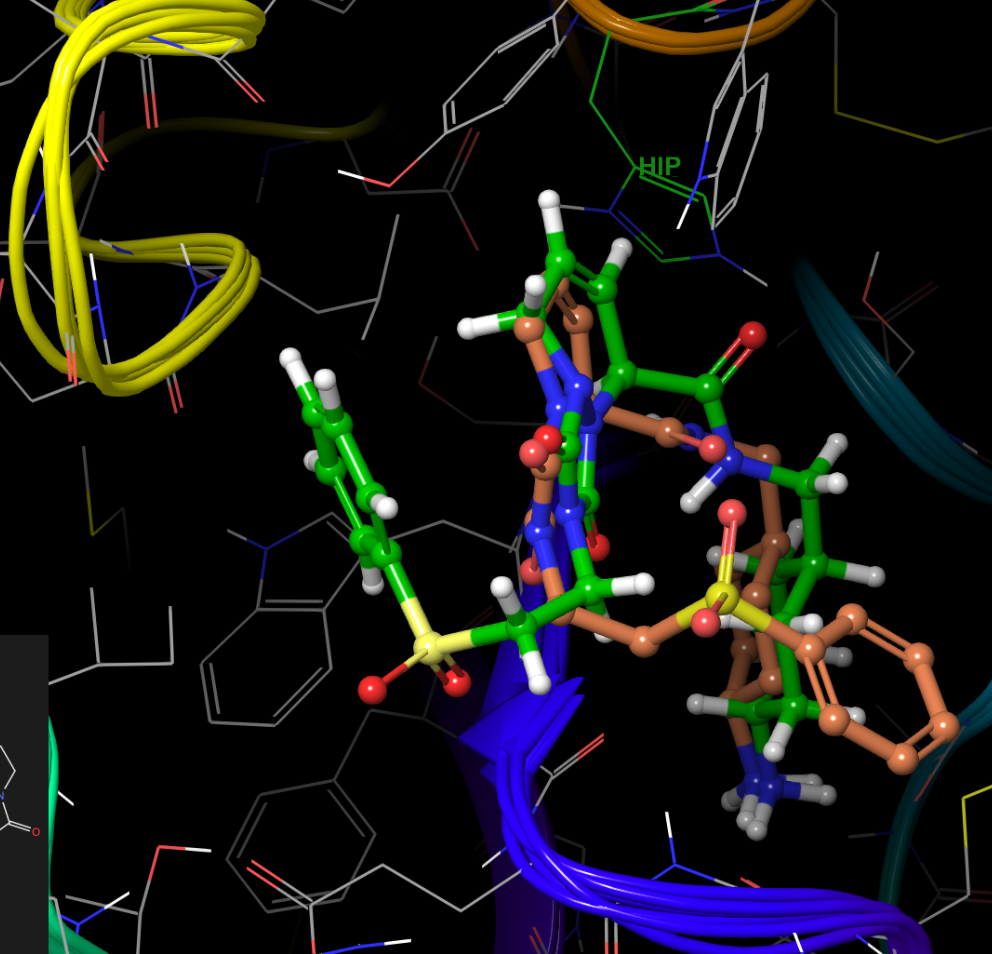
\includegraphics[height=3.8cm]{figures/feature_51_2384.png}
\caption{Thrombin: rotational misorientation. The ligand's bulky substituent is rotated toward the wrong catalytic-pocket residue.}
\end{subfigure}
\hfill
\begin{subfigure}[b]{0.48\textwidth}
\centering
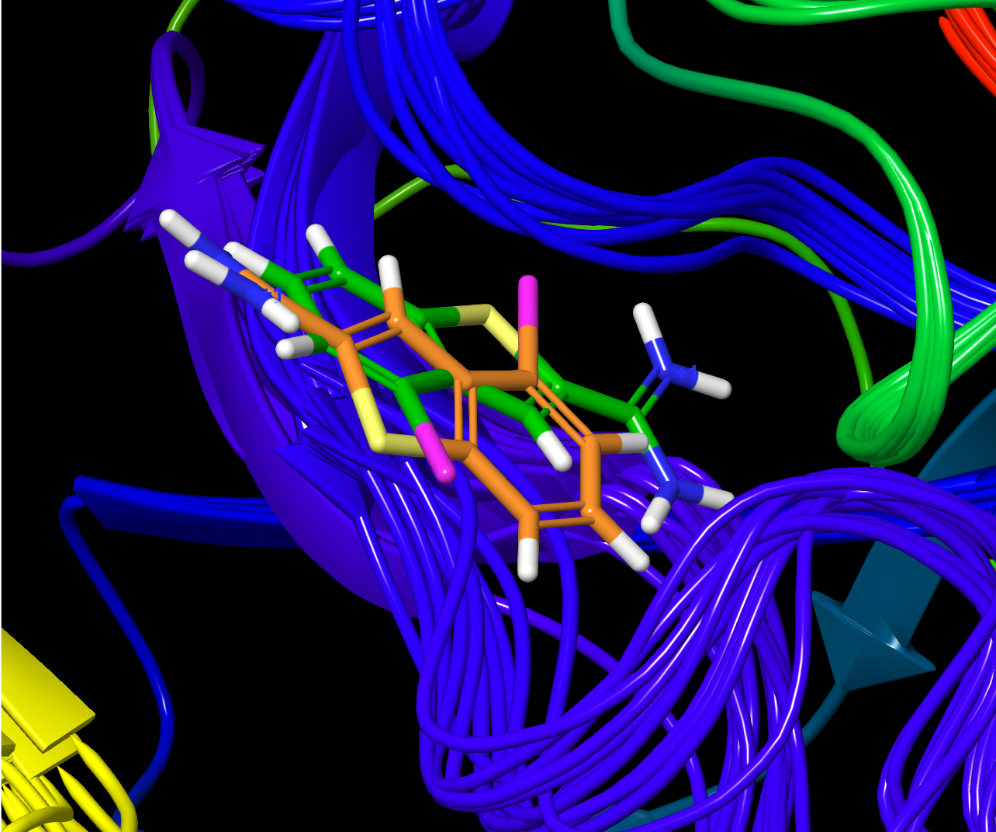
\includegraphics[height=3.8cm]{figures/feature_84_11084.png}
\caption{Urokinase (uPA): translational displacement. The ligand is correctly oriented but shifted within the binding pocket.}
\end{subfigure}
\caption{Representative top-activating poses for the two features discussed in the Conclusion.}
\label{fig:qualitative}
\end{figure}

\end{document}
